\section{Heavily Duplicated Data}
\label{sect:dup}
Knowing that locality has ruled the 
data reduction within individual VM's snapshot backups,
in this section we investigate the dominant factor
of data duplication between VMs. 

Many deduplication study has mentioned that zero-filled
blocks were widely exist, so we count the
zero-filled blocks using the variable 4KB scheme to examine their weights in VM storage.
Table~\ref{tab:zero} shows the total size of zero-filled
blocks divide by data set size.

\begin{table}[htb]
  \centering
    \begin{tabular}{|l|c|}
        \hline
        Data Set & Weight of Zero-filled Blocks\\ \hline
        VOSS & 8.1\% \\ \hline
        DDS & 21.3\% \\
        \hline
    \end{tabular}
    \caption{Weight of zero-filled blocks in our data sets}
    \label{tab:zero}
\end{table}

\emph{Observation 8: User generated data are much less compact than operating system data.}
We see 21.3\% reduction from DDS by removing zero-filled blocks. Consider
that full deduplication can only reduce about 50\% on DDS, this indicates we could
achieve great reduction by simply avoid storing zero-filled blocks in storage system.

Data on OS disks seem much more compact than
user generated contents. However, their duplication may come in from another way.
Consider 99\% of our VM users run either Linux or Windows, and most of them only uses
a small selection of software (e.g., MySQL, Apache), such
operating system and software related data are very likely to be duplicated
across VMs.

We examine this by using the public VM images in Aliyun's cloud environment as a reference.
Every VM is generated from one of the public VM images by copying its data from base image,
so in order to see whether these data are changed after VM usage,
we first split the public images into 4KB variable-sized blocks, then for each type of
OS, we check its 50 VM snapshot backups in VOSS, to see if this data block still exist in all
50 backups. This is a very strict criteria, a data block will only be marked as ``unchanged''
if it appear in all 50 snapshots.

\begin{figure}
  \centering
  %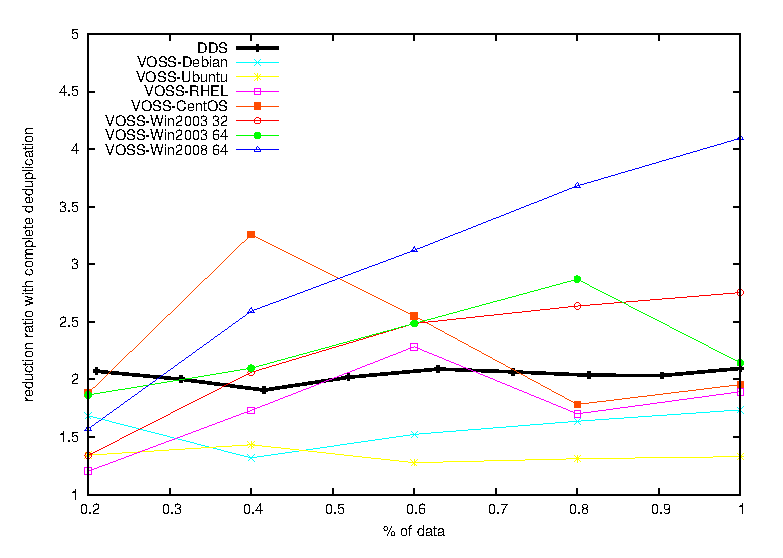
\epsfig{file=dedup_ratio.eps, width=3.2in}
  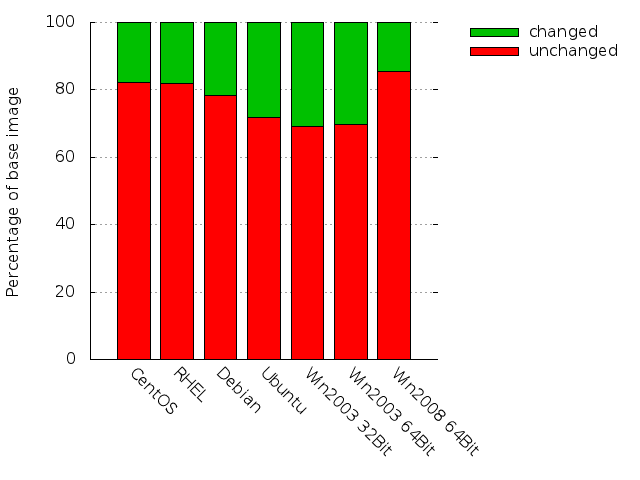
\includegraphics[width=3in,height=2in]{os_subset.png}
  \caption{Data that almost never change in OS disks}
  \label{fig:osdup}
\end{figure}

\emph{Observation 9: OS and software related data rarely change.}
This strongly indicates we should avoid storing such data in any VM's snapshot backups,
if we know they can be obtained from somewhere else. 
In addition, knowing these data are widely used by VMs shall help us developing
fast content delivery scheme for VM migration and snapshot restoration.
